\documentclass[acmlarge]{acmart}
\usepackage[
    type={CC},           % your choice
    modifier={by-sa},    % your choice
    version={4.0},       % your choice
]{doclicense}            % your choice, see \doclicenseThis below


\usepackage{alltt}
%\usepackage{pslatex}
%\usepackage{epigraph}
%\usepackage{verbatim}
\usepackage{latexsym}
\usepackage{array}
%\usepackage{comment}
%\usepackage{makeidx}
%\usepackage{indentfirst}
%\usepackage{verbatim}
%\usepackage{color}
%\usepackage{url}
%\usepackage{xspace}
%\usepackage{hyperref}
%\usepackage{stmaryrd}
\usepackage{amsmath, amsthm}
%\usepackage{graphicx}
%\usepackage{euscript}
\usepackage{mathtools}
%\usepackage{mathrsfs}
%\usepackage{multirow,bigdelim}
%\usepackage{subcaption}
%\usepackage{placeins}
\usepackage{csvsimple}

%\geometry{
%     top=18pt, bottom=14pt, inner=21pt, outer=21pt,
%     paperwidth=5.5in, paperheight=8.5in,
%     }
%     
\settopmatter{printacmref=false}
\fancyfoot{}
 
\makeatletter
\def\@formatdoi#1{}
\def\@permissionCodeOne{miniKanren.org/workshop}
\def\@copyrightpermission{\doclicenseThis} 
\def\@copyrightowner{Copyright held by the author(s).}
\makeatother

\copyrightyear{2019}
\setcopyright{rightsretained}

\acmMonth{8}
\acmArticle{3} % your article number, same as in HotCRP



%% Bibliography style
\bibliographystyle{ACM-Reference-Format}
%% Citation style
%% Note: author/year citations are required for papers published as an
%% issue of PACMPL.
\citestyle{acmauthoryear}   %% For author/year citations


%%%%%%%%%%%%%%%%%%%%%%%%%%%%%%%%%%%%%%%%%%%%%%%%%%%%%%%%%%%%%%%%%%%%%%
%% Note: Authors migrating a paper from PACMPL format to traditional
%% SIGPLAN proceedings format must update the '\documentclass' and
%% topmatter commands above; see 'acmart-sigplanproc-template.tex'.
%%%%%%%%%%%%%%%%%%%%%%%%%%%%%%%%%%%%%%%%%%%%%%%%%%%%%%%%%%%%%%%%%%%%%%


%% Some recommended packages.
\usepackage{booktabs}   %% For formal tables:
                        %% http://ctan.org/pkg/booktabs
\usepackage{subcaption} %% For complex figures with subfigures/subcaptions
                        %% http://ctan.org/pkg/subcaption
\usepackage{multirow}


\usepackage{listings}
\lstdefinelanguage{ocanren}{
keywords={run, conde, fresh, let, in, match, with, when, class, type,
object, method, of, rec, repeat, until, while, not, do, done, as, val, inherit,
new, module, sig, deriving, datatype, struct, if, then, else, open, private, virtual, include, success, failure,
true, false},
sensitive=true,
commentstyle=\small\itshape\ttfamily,
keywordstyle=\ttfamily\textbf,
identifierstyle=\ttfamily,
basewidth={0.5em,0.5em},
columns=fixed,
mathescape=true,
fontadjust=true,
literate={fun}{{$\lambda$}}1 {->}{{$\to$}}3 {===}{{$\equiv$}}1 {=/=}{{$\not\equiv$}}1 {|>}{{$\triangleright$}}3 {\\/}{{$\vee$}}2 {/\\}{{$\wedge$}}2 {^}{{$\uparrow$}}1,
morecomment=[s]{(*}{*)}
}

\lstset{
%mathescape=true,
%basicstyle=\small,
%identifierstyle=\ttfamily,
%keywordstyle=\bfseries,
%commentstyle=\scriptsize\rmfamily,
%basewidth={0.5em,0.5em},
%fontadjust=true,
language=ocanren
}

\newcommand{\lstquot}[1]{``\lstinline{#1}''}
\newcommand{\sembr}[1]{\llbracket{#1}\rrbracket}
\newcommand\false{$f\!alse$}
\newcommand\myif{i\!f}


\def\transarrow{\xrightarrow}
\newcommand{\setarrow}[1]{\def\transarrow{#1}}

\def\padding{\phantom{X}}
\newcommand{\setpadding}[1]{\def\padding{#1}}

\def\subarrow{}
\newcommand{\setsubarrow}[1]{\def\subarrow{#1}}

\newcommand{\trule}[2]{\dfrac{#1}{#2}}
\newcommand{\crule}[3]{\dfrac{#1}{#2},\;{#3}}
\newcommand{\withenv}[2]{{#1}\vdash{#2}}
\newcommand{\trans}[3]{{#1}\transarrow{\padding{\textstyle #2}\padding}\subarrow{#3}}
\newcommand{\ctrans}[4]{{#1}\transarrow{\padding#2\padding}\subarrow{#3},\;{#4}}
\newcommand{\llang}[1]{\mbox{\lstinline[mathescape]|#1|}}
\newcommand{\pair}[2]{\inbr{{#1}\mid{#2}}}
\newcommand{\inbr}[1]{\left<{#1}\right>}
\newcommand{\highlight}[1]{\color{red}{#1}}
%\newcommand{\ruleno}[1]{\eqno[\scriptsize\textsc{#1}]}
\newcommand{\ruleno}[1]{\mbox{[\textsc{#1}]}}
\newcommand{\rulename}[1]{\textsc{#1}}
\newcommand{\inmath}[1]{\mbox{$#1$}}
\newcommand{\lfp}[1]{fix_{#1}}
\newcommand{\gfp}[1]{Fix_{#1}}
\newcommand{\vsep}{\vspace{-2mm}}
\newcommand{\supp}[1]{\scriptsize{#1}}
\renewcommand{\sembr}[1]{\llbracket{#1}\rrbracket}
\newcommand{\cd}[1]{\texttt{#1}}
\newcommand{\free}[1]{\boxed{#1}}
\newcommand{\binds}{\;\mapsto\;}
\newcommand{\dbi}[1]{\mbox{\bf{#1}}}
\newcommand{\sv}[1]{\mbox{\textbf{#1}}}
\newcommand{\bnd}[2]{{#1}\mkern-9mu\binds\mkern-9mu{#2}}
\newcommand{\meta}[1]{{\mathcal{#1}}}
\newcommand{\dom}[1]{\mathtt{dom}\;{#1}}
%\newcommand{\primi}[2]{\mathbf{#1}\;{#2}}
\renewcommand{\dom}[1]{\mathcal{D}om\,({#1})}
\newcommand{\ran}[1]{\mathcal{VR}an\,({#1})}
\newcommand{\fv}[1]{\mathcal{FV}\,({#1})}
\newcommand{\tr}[1]{\mathcal{T}r_{#1}}
\newcommand{\diseq}{\not\equiv}
\newcommand{\reprfunset}{\mathcal{R}}
\newcommand{\reprfun}{\mathfrak{f}}
\newcommand{\cstore}{\Omega}
\newcommand{\cstoreinit}{\cstore_\epsilon^{init}}
\newcommand{\csadd}[3]{add(#1, #2 \diseq #3)}  %{#1 + [#2 \diseq #3]}
\newcommand{\csupdate}[2]{update(#1, #2)}  %{#1 \cdot #2}
\newcommand{\primi}[1]{\mathbf{#1}}
\newcommand{\sem}[1]{\llbracket #1 \rrbracket}
\newcommand{\ir}{\ensuremath{\mathcal{S}\mathcal{W}}}

\let\emptyset\varnothing
\let\eps\varepsilon

\sloppy 




\begin{document}

\title[Relational Synthesis of Pattern Matching]{Relational Synthesis for Pattern Matching}    

\titlenote{This work was partially suppored by the grant 18-01-00380 from The Russian Foundation for Basic Research} %% \titlenote is optional;


\author{Dmitry Kosarev}
\email{Dmitrii.Kosarev@pm.me}

\author{Dmitry Boulytchev}
\email{dboulytchev@math.spbu.ru}    

\affiliation{
  \institution{Saint Petersburg State University}
  \country{Russia}                   
}

\affiliation{
  \institution{JetBrains Research}   
  \country{Russia}                   
}


%% Abstract
%% Note: \begin{abstract}...\end{abstract} environment must come
%% before \maketitle command
\begin{abstract}
Effective compilation of pattern matching is important part in a compiler of typed functional language.  We address it via relational synthesis, the algorithm is searching for compiled representation which behaves well on full but finite set of examples and which is minimal. We also describe how to generate full set of examples and our  criteria of minimalism. The approach using relational synthesis seems to be more asily extensible than the default ones.
\end{abstract}


%% 2012 ACM Computing Classification System (CSS) concepts
%% Generate at 'http://dl.acm.org/ccs/ccs.cfm'.
\begin{CCSXML}
<ccs2012>
<concept>
<concept_id>10011007.10011006.10011008.10011009.10011015</concept_id>
<concept_desc>Software and its engineering~Constraint and logic languages</concept_desc>
<concept_significance>500</concept_significance>
</concept>
<concept>
<concept_id>10011007.10011006.10011041.10011047</concept_id>
<concept_desc>Software and its engineering~Source code generation</concept_desc>
<concept_significance>500</concept_significance>
</concept>
</ccs2012>
\end{CCSXML}

\ccsdesc[500]{Software and its engineering~Constraint and logic languages}
\ccsdesc[500]{Software and its engineering~Source code generation(FIXME)}
%% End of generated code


%% Keywords
%% comma separated list
\keywords{relational programming, relational interpreters, search problems}  %% \keywords are mandatory in final camera-ready submission


%% \maketitle
%% Note: \maketitle command must come after title commands, author
%% commands, abstract environment, Computing Classification System
%% environment and commands, and keywords command.
\maketitle

\thispagestyle{empty}

\section{Introduction}


  \begin{comment}
We implemented the synthesis framework using \textsc{OCanren}~--- an embedding of \textsc{miniKanren} into \textsc{OCaml}~\cite{ocanren},~---
 and evaluated it on the set of benchmarks, reported in the previous works on \emph{ad-hoc} algorithms for pattern matching
 code generation~\cite{maranget2001,maranget2008}. In comparison with a simplified setting, presented above, our implementation
 deals with a more elaborate pattern matching problem~--- in particular, we support \emph{guard expressions}, name bindings in
 patterns and incorporate a deterministic top-down matching strategy, which is common in functional languages.
 
 Initially, our synthesis did not demonstrate good results. However, we applied the following techniques to improve both the performance
 and the quality of synthesized programs:
 
 \begin{itemize}
 \item we restricted the shape of scrutinees using type information;
 \item we utilized tabling to memoize repeating search steps;
 \item we implemented a pruning technique, which makes the search stop exploring a certain branch if the program, synthesized so far,
   contains too much nesting constructs (this factor can be precomputed by patterns analysis).
 \end{itemize}
 
 With these adjustments, our synthesis framework in a negligible time provides the same results as those reported in the previous works.
 Our future steps include extending the pattern matching language to completely match that of \textsc{OCaml} (for
 now we do not support GADTs), integrate the synthesis into the existing \textsc{OCaml} compiler and evaluate it on a
 set of real-world programs. Another direction is extending the pattern matching language to incorporate features which
 are known to be hard, tedious or error-prone to implement (for example, non-linear patterns).
 
\end{comment}


\begin{comment}

Algebraic data types are essential for typed functional programming and it's difficult to imagine effective compiler without effective compilation of pattern matching. 
There are a few different approaches for compiling pattern mathcing. GHC is using influential paper~\cite{Jones1987}, OCaml is currently based on~\cite{maranget2001} although a work~\cite{maranget2008} can slightly improve effectiveness of generated code. 

Also there are a number of possible extensions of pattern matching itself (guards, non-linear patterns, active patterns) and extensions of possible matchable values (polymorphic variants in OCaml, for example). Although having all these extensions can be helpful for programming in practice, they can complicate compilation schema or make it very difficult to generate effective code. Supporting a large number  of extensions can seriously complicate compiler's implementation too.

We present an approach to pattern matching code generation based on application of relational programming~\cite{TRS,WillThesis} and, in
 particular, relational interpreters~\cite{unified}. We expect that our approach can compile pattern mathcing to competitive code and will be easier to support during adding of new pattern matching extensions.
 
\end{comment}
 We use a \emph{relational interpreter} for $\ir$
 
 \[
 eval^o_{\ir}\, (s, p, i)
 \]
 
 Here $s$ and $i$ have the same meaning as in declarative semantics description, $p\in\ir$~--- a syntactic representation of
 a program in $\ir$. The relation $eval^o_{\ir}$ encodes the operational semantics of $\ir$; it holds, if
 evaluating $p$ for $s$ returns $i$. Being relational interpreter, however, $eval^o_{\ir}$ is capable of solving a
 synthesis problem: by a scrutinee $s$ and a number $i$ calculate a program $p$ which makes the relation to hold.
 Within this setting, we can formulate the pattern-matching synthesis problem as follows: \emph{for a given ordered list of patterns $ps$ find a program $p$, such that}
 
 \[
 \forall s\in\mathcal{V},\,\exists i,\,eval^o_{\ir}\, (s, p, i) \wedge\, match (s, ps, i)
 \]
 
 It is rather problematic to directly solve this synthesis problem with existing \textsc{miniKanren} implementations as
 they provide a rather limited support for universal quantification~\cite{eigen,moiseenko}. However, in our concrete
 case there is a simple way to alleviate this problem. Indeed, we may replace universal quantification over $i$ by
 a finite conjunction, as the length of $ps$ is known at the synthesis time. As for the quantification over $s$, for
 any concrete $ps$ we may precompute a \emph{complete set of examples} $\mathcal{E}(ps)\subseteq\mathcal{V}$ with the following
 property:
 
 \[
 \forall i\in\mathbb{N},\,(\forall s\in\mathcal{E}(ps),\,match\, (s, ps, i) \Leftrightarrow \forall s\in\mathcal{V},\,match\, (s, ps, i))
 \]
 
 It easy to see, that for arbitrary $ps$ there exists a finite complete set of examples (indeed, any pattern describes the ``shape''
 of a scrutinee up to some finite depth, beyond which all scrutinees become indistinguishable). Thus, for a given $ps$ we may
 completely eliminate the quantification, reformulating the synthesis problem as
 
 \[
 \bigwedge_{i\in[1\dots|ps|]}\,\bigwedge_{s\in\mathcal{E}(ps)} (eval^o_{\ir}\, (s, p, i) \wedge match\, (s, ps, i))
 \]
 
 We implemented the synthesis framework using \textsc{OCanren}~--- an embedding of \textsc{miniKanren} into \textsc{OCaml}~\cite{ocanren},~---
 and evaluated it on the set of benchmarks, reported in the previous works on \emph{ad-hoc} algorithms for pattern matching
 code generation~\cite{maranget2001,maranget2008}. In comparison with a simplified setting, presented above, our implementation
 deals with a more elaborate pattern matching problem~--- in particular, we support \emph{guard expressions}, name bindings in
 patterns and incorporate a deterministic top-down matching strategy, which is common in functional languages.
 
 Initially, our synthesis did not demonstrate good results. However, we applied the following techniques to improve both the performance
 and the quality of synthesized programs:
 
 \begin{itemize}
 \item we restricted the shape of scrutinees using type information;
 \item we utilized tabling to memoize repeating search steps;
 \item we implemented a pruning technique, which makes the search stop exploring a certain branch if the program, synthesized so far,
   contains too much nesting constructs (this factor can be precomputed by patterns analysis).
 \end{itemize}
 
 With these adjustments, our synthesis framework in a negligible time provides the same results as those reported in the previous works.
 Our future steps include extending the pattern matching language to completely match that of \textsc{OCaml} (for
 now we do not support GADTs), integrate the synthesis into the existing \textsc{OCaml} compiler and evaluate it on a
 set of real-world programs. Another direction is extending the pattern matching language to incorporate features which
 are known to be hard, tedious or error-prone to implement (for example, non-linear patterns).
 
 \begin{comment}
 
 
 Real world modern compilers are obliged to address a few problems which are NP-complete and hence can't have effective
 algorithm to solve them. So, compilers use semi-optimal algorithms to find a decent solution. Optimal algorithms require
 brute force search to get the best solution and  affect compilation speed negatively. In this work we apply relational
 programming -- a convenient DSL for implementing search -- to compilation of pattern matching, one of a kind hard problems for compiler.
 
 The task of compiling pattern matching for typed languages is well presented in literature~\cite{maranget2001,maranget2008}.
 
 
 We test approach on simplified source language $PM$ where scrutinee is a value $\in\mathcal{V}$ of algebraic data type, only wildcards
 and nested constructors are allowed as patterns $\mathcal{P}$ and right hand side of clause is its index. The source language is easy
 extendable by pattern variables and optional pattern guards that test subterms of scrutinee using a function. The semantics of $PM$
 is a function from concrete scrutinee $s$, concrete patterns $pats$ and concrete guards $gs$ to clause indexes, and is denoted
 as $\sem{s,pats,gs}_{PM} = i$.
 
 Compilation scheme translates sentences from $PM$ to $\ir$ language which has constructions for clause indexes and conditions which
 test matchable values for specific constructor. Matchable values can be either a scrutinee, or a projection of matchable value that
 returns one of its field indexed by natural numbers. $\ir$ language is easy extendable by tests for fixed number of pattern guards.
 The semantics is straightforward and is denoted by $\sem{\cdot}_{\ir}$.
 
 We deal with a task of compiling pattern matching as it is a synthesis problem. The goal of algorithm is to synthesize $ideal_\ir$
 for concrete patterns $pats$ and guards that, firstly, will behave the same as original pattern matching for any possible
 scrutinee $s$. Secondly, we want shortest solution because short code usually runs faster. Relational programming~\cite{OCanren}
 will help with that because it has a tendency to generate short answers earlier, although this tendency is not strict.
 
 $$
 \forall s:\; \sem{s; ideal_\ir}_\ir = \sem{s;pats}_{PM}
 $$
 
 To eliminate universal quantifier we use the following observation: for \emph{finite} amount of patterns of \emph{finite} height
 we can generate \emph{finite} amount of examples to test pattern matching semantics. In examples, very deep subterms can have
 any value because they will not be tested during pattern matching. We can reformulate synthesis problem as follows:
 
 $$
 \mid  Examples\mid < \infty\quad \land\quad \left(\forall e \; (e\in Examples)\quad\land \quad\left( \sem{e; ideal_\ir}_\ir = \sem{e;pats}_{PM}\right)\right)
 $$
 
 For plain ADT the approach will generate required examples in finite time, but for GADTs it can diverge because inhabitancy problem
 is semi-decidable~\cite{garrigue2017gadts}(chapter 5). Inhabitants generation as well as synthesis algorithm is
 implemented\footnote{\url{https://github.com/Kakadu/pat-match/}} using relational programming.
 
 Presented approach is good as general description of an idea but require a few tweaks to start working, for example, on presented
 sample~\ref{fig:example1} . Firstly, synthesis procedure in a way as it is described doesn't take types into account, so it is
 useful to give hints about which parts of scrutinee should be checked for which constructors. Second observation says that we
 run $\sem{\cdot}_\ir$ in concrete direction, so it is possible to check periodically count of \texttt{IfTag} constructors in
 result value and prune branches where it becomes too big. Thirdly, synthesis query generates a lot of similar queries, and
 we use tabling to speedup search. All three observations are important, removing one of them leads to visible performance degradation.
 
 The optimal (two \texttt{IfTag}'s) and the semi-optimal solution (three \texttt{IfTag}'s) for~\ref{fig:example1} are described
 in~\cite{maranget2008}. Current implementation generates semi-optimal solution as 28th answer. Before that it generates optimal
 solution (and it's equivalents) three times, other 24 answers are longer and less useful. All tasks (example generation, synthesis
 and printing answers) take 3 seconds, which is unfortunate.
 
 Shortly, we present following contributions
 \begin{itemize}
 \item Code synthesis for pattern matching works after implementing \emph{three optimizations} above.
 \item GADTs, pattern binding and guards works for simple examples, the approach is easy extendable by them.
 \end{itemize}
 
 Future work is
 \begin{itemize}
 \item Discover other optimizations and enable current ones automatically using type information (at the moment we patched synthesis
   algorithm manually for concrete example).
 \item When current implementation tests for \texttt{cons} tag it can't propagate constraint that tag equals to \texttt{nil} to
   the \texttt{else} branch, which partially explains why branch pruning is so useful.
 \item Algorithm for inhabitant generation requires proper formulation and proof.
 \item Apply current synthesis procedure for exhaustiveness checking which will give us \emph{single} procedure for compilation and exhaustiveness checking.
 \item Test the approach on real world problems (embedding to OCaml compiler).
 \end{itemize}
 
 
 \begin{figure}[t]
   \[
   \begin{array}{rcll}
     \mathcal{C} & = & \{ C_1^{k_1}, \dots, C_n^{k_n} \}    &\mbox{(constructors)} \\
     \mathcal{V} & = & \mathcal{C}\,\mathcal{V}^*        &\mbox{(values)}       \\
     \mathcal{P} & = & \_ \mid \mathcal{C}\,\mathcal{P}^*&\mbox{(patterns)}     \\
     \mathcal{M} & = & \bullet \mid \mathcal{M} [\mathbb{N}]&
 
   \end{array}
   \]
 \end{figure}
 
 \begin{figure}
 \centering
 \begin{minipage}{.7\textwidth}
   \centering
 \begin{align*}
 \mathcal{C} =&\; \{ C_1^{k_1}, \dots, C_n^{k_n} \} \\
 \mathcal{V} =&\;  \mathcal{C}\ \mathcal{V}^*\\
 \mathcal{M} =&\;  \mathcal{S} \\
           \mid\; &\; \text{\texttt{Field}}\;  \mathcal{M}\times  \mathbb{N}\\
 \mathcal{P} =&\;  \text{\texttt{Wildcard}} \\
           \mid\; &\; \text{\texttt{Var}}\  Name\\
           \mid\; &\; \text{\texttt{PConstructor}}\  \mathcal{C}\times  \mathcal{P}^*\\
 \ir  =&\; \text{\texttt{Int}}\  \mathbb{N} \\
 %           \mid\; &\;\mathcal{S} \\
            \mid\; &\; \text{\texttt{IfTag}}\; \mathcal{C}\times \mathcal{M}\times \ir\times \ir\\
            \mid\; &\; \text{\texttt{IfGuard}}\ \mathbb{N}\times (Name\times \mathcal{M})^*\times \ir\times \ir\\
 Clause =&\;  \mathcal{P} \times \mathbb{N}? \times \ir
 \end{align*}
   \captionof{figure}{Structure of $PM$ and \ir languages}
 %  \label{fig:test1}
 \end{minipage}%
 \begin{minipage}{.3\textwidth}
   \centering
 \begin{lstlisting}[language=ocaml]
 match s with 
 | ([], _)     -> 1
 | (_, [])     -> 2
 | (_::_,_::_) -> 3
 \end{lstlisting}
   \captionof{figure}{Simple example of pattern matching problem from~\cite{maranget2008}}
 \label{fig:example1}
 \end{minipage}
 \end{figure}
 
 \end{comment}
 

\section{Related Works}
\label{sec:related_works}

The non-commutativity of conjunction evaluation in miniKanren is a well-known problem. In~\cite{WillThesis} some language
extensions are discussed, which, presumably, can be used to provide the commutativity. They include both simple enumeration
of conjunct orders and more advanced techniques, based on a combination of tabling, parallel goal evaluation, and continuations.
However, by now none of these proposals were implemented or evaluated. The tabling technique, described in the same work, can
indeed be used to provide the convergence of some queries, but it deals with the problems, orthogonal to the non-commutativity,
and, thus, does not heal the queries, which we do (but heals some other cases, like divergence of path-finding queries for
graphs with cycles, which we do not). 

For a number of problems some \emph{ad-hoc} refutationally complete solutions were already presented before. For example,
in~\cite{TRS} a number of relations for binary arithmetics, implemented using the idea of bounding the sizes of terms, are
presented. In a follow-up paper~\cite{KiselyovArithmetic} this technique is explained in details, and the proof of refutational
completeness is given. Unfortunately, the specifications, written using this technique, are verbose and
hard to understand, and the implementation requires insight. Our improvement, on the other hand, makes it possible to stick
with the simplest definitions, and althought we do not provide a proof of refutational completeness for each case, for the
majority of realistic queries they converge and demonstrate the same performance, as those, implemented with advanced methods.

In a broader context of logical programming the problem of search convergence/termination was addressed multiple
times. However, it is rather hard to establish a direct correspondence between our proposal and the reported results,
since they were developed for essentially different language. For example, in~\cite{OLDresolution} a tabling-based
improvement of a resolution-based search~--- OLDT resolution~--- is described, and a complete search strategy is developed.
However, in miniKanren the original search is already complete, and we address rather a different issue. We can speculate,
that OLDT resolution roughly corresponds to the miniKanren with tabling and, thus, posesses the same properties, and relates to
our proposal in a similar manner.



\section{The Pattern Matching Synthesis Problem}

We describe here a simplified view on pattern matching which does not incorporate some practically important aspects of the construct such as
name bindings in patterns, guards or even semantic actions in branches. In a purified form, however, it  represents the essence of pattern
matching as an ``inspect-and-branch'' procedure. Other features can be easily added later once a solution for the essential part of the problem
is found.

First, we introduce a finite set of \emph{constructors} $\mathcal C$, equipped with arities, a set of values $\mathcal{V}$
and a set of patterns $\mathcal{P}$:
 
\[
 \begin{array}{rcll}
    \mathcal{C} & = & \{ C_1^{k_1}, \dots, C_n^{k_n} \}\\
    \mathcal{V} & = & \mathcal{C}\,\mathcal{V}^*\\  
    \mathcal{P} & = & \_ \mid \mathcal{C}\,\mathcal{P}^*
 \end{array}
\]

We define a matching of a value $v$ (\emph{scrutinee}) against an ordered non-empty sequence of patterns $p_1,\dots,p_k$ by means of the following
relation

\[
\setarrow{\xrightarrow}
\trans{\inbr{v;\,p_1,\dots,p_k}}{}{i},\,1\le i\le k+1
\]

which gives us the index of the leftmost matched pattern or $k+1$ if no such pattern exists. We use an auxiliary relation $\inbr{;}\subseteq\mathcal{V}\times\mathcal{P}$
to specify the notion of a value matched by an individual pattern (see Fig.~\ref{fig:match1pat}). The rule \ruleno{Wildcard} says that
a wildcard pattern ``\_'' matches any value, and \ruleno{Constructor} specifies that a constructor pattern matches exactly those values which
have the same constructor at the top level and all subvalues matched by corresponding subpatterns. The definition of ``$\xrightarrow{}{\!\!}$'' is
shown on Fig.~\ref{fig:matchpatts}. An auxiliary relation
 ``$\xrightarrow{}{}_{\!\!*}$'' 
is introduced to specify the left-to-right matching strategy, and we
use current index as an environment. An important rule, $\ruleno{MatchOtherwise}$ specifies that if we exhausted all the patterns with no matching we stop with
the current index (which in this case is equal to the number of patterns plus one).

\begin{figure}[t]
   \renewcommand*{\arraystretch}{2}
   \[
   \begin{array}{cr}
     \inbr{v;\,\_} & \ruleno{Wildcard} \\
     \trule{\forall i\;\inbr{v_i;\,p_i}}{\inbr{C^k\,v_1\dots v_k;\,C^k\,p_1\dots p_k}},\,k\ge 0 & \ruleno{Constructor}
   \end{array}
   \]
   \caption{Matching against a single pattern}
   \label{fig:match1pat}
\end{figure}

\begin{figure}[t]
   \renewcommand*{\arraystretch}{3}
   \setarrow{\xrightarrow}
   \setsubarrow{_*}
   \[
   \begin{array}{cr}
     \trule{\inbr{v;\,p_1}}
           {\withenv{i}{\trans{\inbr{v;\,p_1,\dots,p_k}}{}{i}}} & \ruleno{MatchHead}\\
     \trule{\neg\inbr{v;\,p_1}\qquad\withenv{i+1}{\trans{\inbr{v;\,p_2,\dots,p_k}}{}{j}}}
           {\withenv{i}{\trans{\inbr{v;\,p_1,\dots,p_k}}{}{j}}} & \ruleno{MatchTail}\\
     \withenv{i}{\trans{\inbr{v;\,\varepsilon}}{}{i}} & \ruleno{MatchOtherwise}\\
     \trule{\withenv{1}{\trans{\inbr{v;\,p_1,\dots,p_k}}{}{i}}}
           {\setsubarrow{}\trans{\inbr{v;\,p_1,\dots,p_k}}{}{i}} & \ruleno{Match}
   \end{array}
   \]
   \caption{Matching against an ordered sequence of patterns}
   \label{fig:matchpatts}
\end{figure}

The relation ``$\xrightarrow{}{}\!\!$'' gives us a \emph{declarative} semantics of pattern matching. Since we are interested in
synthesizing implementations, we need a \emph{programmatical} view on the same problem. Thus, we introduce a language $\mathcal S$
(the ``switch'' language) of test-and branch constructs:

\[
\begin{array}{rccl}
  \mathcal M & = &       & \bullet \\
             &   & \mid  & \mathcal M\,[\mathbb{N}] \\
  \ir        & = &       & \primi{return}\,\mathbb{N} \\
             &   & \mid  & \primi{switch}\;\mathcal{M}\;\primi{with}\; [\mathcal{C}\; \primi{\rightarrow}\; \ir]^*\;\primi{otherwise}\;\ir
\end{array}
\]
 
Here $\mathcal{M}$ stands for a \emph{matching expression}, which is either a reference to a scrutinee ``$\bullet$'' or
a (multiply) indexed subexpression of a scrutinee. Programs in the switch language can discriminate on the
structure of matching expressions, testing their top-level constructors and eventually returning natural numbers as results.
The switch language is similar to the intermediate representations for pattern matching code used in 
previous works on pattern matching implementation~\cite{maranget2001,maranget2008}, and switch programs are analogous to
\emph{decision trees}.

The semantics of the switch language is given by mean of relations ``$\xrightarrow{}{}_{\!\!\!\mathcal M}$'' and ``$\xrightarrow{}{}_{\!\!\mathcal S}$''
(see Fig.~\ref{fig:matchexpr} and \ref{fig:test-and-branch}). The first one describes the semantics of matching expression, while
the second describes the semantics of the switch language itself. In both cases the scrutinee $v$ is used as an environment ($v\vdash$).


\begin{figure}[t]
  \renewcommand*{\arraystretch}{2}
  \setarrow{\xrightarrow}
  \setsubarrow{_{\mathcal M}}
  \[
  \begin{array}{cr}
    \withenv{v}{\trans{\bullet}{}{v}} & \ruleno{Scrutinee} \\
    \trule{\withenv{v}{\trans{m}{}{C^k v_1\dots v_k}}}{\withenv{v}{\trans{m[i]}{}{v_i}}} & \ruleno{SubMatch} 
  \end{array}
  \]
  \caption{Semantics of matching expression}
  \label{fig:matchexpr}
\end{figure}

\begin{figure}[t]
  \setarrow{\xrightarrow}
  \setsubarrow{_{\mathcal S}}
  \[
  \begin{array}{cr}
    \withenv{v}{\trans{\primi{return}\;i}{}{i}} & \ruleno{Return}\\[10mm]
    
    \trule{\renewcommand*{\arraystretch}{1}
           \begin{array}{c}        
              {\setsubarrow{_{\mathcal M}}\withenv{v}{\trans{m}{}{C^k\ v_1 \dots v_k}}} \\
              \withenv{v}{\trans{s}{}{i}}
           \end{array}
          }    
          {\withenv{v}{\trans{\primi{switch}\;m\;\primi{with}\;[C^k\to s]s^*\;\primi{otherwise}\;s^\prime}{}{i}}} & \ruleno{SwitchMatched}\\[10mm]
          
    \trule{\renewcommand*{\arraystretch}{1}
           \begin{array}{c}        
             {\setsubarrow{_{\mathcal M}}\withenv{v}{\trans{m}{}{D^n\  v_1 \dots v_n}}}\\
             C^k\ne D^n\\
             \withenv{v}{\trans{\primi{switch}\;m\;\primi{with}\;s^*\;\primi{otherwise}\;s^\prime}{}{i}}
           \end{array}
          }
          {\withenv{v}{\trans{\primi{switch}\;m\;\primi{with}\;[C^k\to s]s^*\;\primi{otherwise}\;s^\prime}{}{i}}} & \ruleno{SwitchNotMatched}\\[10mm]
          
    \trule{\withenv{v}{\trans{s}{}{i}}}{\withenv{v}{\trans{\primi{switch}\;m\;\primi{with}\;\varepsilon\;\primi{otherwise}\;s}{}{i}}} & \ruleno{SwitchOtherwise}
  \end{array}
  \]
  \caption{Semantics of switch programs}
  \label{fig:test-and-branch}
\end{figure}

The following observations can be easily proven by structural induction.

\begin{Observation}
  For arbitrary pattern the set of matching values is non-empty:

  \[
  \forall p\in\mathcal P : \{v\in\mathcal V\mid \inbr{v;\,p}\}\ne\emptyset
  \]
\end{Observation}

\begin{Observation}
  Relations ``$\xrightarrow{}{}\!\!\!$'' and ``$\xrightarrow{}{}_{\!\!\mathcal S}$'' are functional and deterministic respectively:

  \[
  \setarrow{\xrightarrow}
  \begin{array}{rcl}
    \forall p_1,\dots,p_k\in\mathcal P,\,\forall v\in \mathcal V,\,\forall \pi\in\mathcal S & : & |\{i\in\mathbb N\mid \trans{\inbr{v;\,p_1,\dots,p_k}}{}{i}\}|=1 \\
                                                                 &  & {\setsubarrow{_{\mathcal S}}|\{i\in\mathbb N\mid \withenv{v}{\trans{\pi}{}{i}}\}|\le 1}
  \end{array}
  \]
\end{Observation}

With these definitions, we can formulate the \emph{pattern matching synthesis problem} as follows: for a given ordered sequence of patterns $p_1,\dots,p_k$ find
a switch program $\pi$, such that

\[
\setarrow{\xrightarrow}
\forall v\in \mathcal V,\; \forall 1\le i\le n+1 : \trans{\inbr{v;\,p_1,\dots,p_n}}{}{i}\Longleftrightarrow{\setsubarrow{_{\mathcal S}}\withenv{v}{\trans{\pi}{}{i}}}\eqno{(\star)}
\]

In other words, program $\pi$ delivers a correct and complete implementation for pattern matching.

Algebraic data types are essential for typed functional programming and it's difficult to imagine effective compiler without effective compilation of pattern matching. 
There are a few different approaches for compiling pattern mathcing. GHC is using influential paper~\cite{Jones1987}, OCaml is currently based on~\cite{maranget2001} although a work~\cite{maranget2008} can slightly improve effectiveness of generated code. 

Also there are a number of possible extensions of pattern matching itself (guards, non-linear patterns, active patterns) and extensions of possible matchable values (polymorphic variants in OCaml, for example). Although having all these extensions can be helpful for programming in practice, they can complicate compilation schema or make it very difficult to generate effective code. Supporting a large number  of extensions can seriously complicate compiler's implementation too.

We present an approach to pattern matching code generation based on application of relational programming~\cite{TRS,WillThesis} and, in
 particular, relational interpreters~\cite{unified}. We expect that our approach can compile pattern mathcing to competitive code and will be easier to support during adding of new pattern matching extensions.
 
 We use a \emph{relational interpreter} for $\ir$
 
 \[
 eval^o_{\ir}\, (s, p, i)
 \]
 
 Here $s$ and $i$ have the same meaning as in declarative semantics description, $p\in\ir$~--- a syntactic representation of
 a program in $\ir$. The relation $eval^o_{\ir}$ encodes the operational semantics of $\ir$; it holds, if
 evaluating $p$ for $s$ returns $i$. Being relational interpreter, however, $eval^o_{\ir}$ is capable of solving a
 synthesis problem: by a scrutinee $s$ and a number $i$ calculate a program $p$ which makes the relation to hold.
 Within this setting, we can formulate the pattern-matching synthesis problem as follows: \emph{for a given ordered list of patterns $ps$ find a program $p$, such that}
 
 \[
 \forall s\in\mathcal{V},\,\forall i\in\mathbb{N},\,eval^o_{\ir}\, (s, p, i) \wedge\, match (s, ps, i)
 \]
 
 It is rather problematic to directly solve this synthesis problem with existing \textsc{miniKanren} implementations as
 they provide a rather limited support for universal quantification~\cite{eigen,moiseenko}. However, in our concrete
 case there is a simple way to alleviate this problem. Indeed, we may replace universal quantification over $i$ by
 a finite conjunction, as the length of $ps$ is known at the synthesis time. As for the quantification over $s$, for
 any concrete $ps$ we may precompute a \emph{complete set of examples} $\mathcal{E}(ps)\subseteq\mathcal{V}$ with the following
 property:
 
 \[
 \forall i\in\mathbb{N},\,(\forall s\in\mathcal{E}(ps),\,match\, (s, ps, i) \Leftrightarrow \forall s\in\mathcal{V},\,match\, (s, ps, i))
 \]
 
 It easy to see, that for arbitrary $ps$ there exists a finite complete set of examples (indeed, any pattern describes the ``shape''
 of a scrutinee up to some finite depth, beyond which all scrutinees become indistinguishable). Thus, for a given $ps$ we may
 completely eliminate the quantification, reformulating the synthesis problem as
 
 \[
 \bigwedge_{i\in[1\dots|ps|]}\,\bigwedge_{s\in\mathcal{E}(ps)} (eval^o_{\ir}\, (s, p, i) \wedge match\, (s, ps, i))
 \]
 
 We implemented the synthesis framework using \textsc{OCanren}~--- an embedding of \textsc{miniKanren} into \textsc{OCaml}~\cite{ocanren},~---
 and evaluated it on the set of benchmarks, reported in the previous works on \emph{ad-hoc} algorithms for pattern matching
 code generation~\cite{maranget2001,maranget2008}. In comparison with a simplified setting, presented above, our implementation
 deals with a more elaborate pattern matching problem~--- in particular, we support \emph{guard expressions}, name bindings in
 patterns and incorporate a deterministic top-down matching strategy, which is common in functional languages.
 
 Initially, our synthesis did not demonstrate good results. However, we applied the following techniques to improve both the performance
 and the quality of synthesized programs:
 
 \begin{itemize}
 \item we restricted the shape of scrutinees using type information;
 \item we utilized tabling to memoize repeating search steps;
 \item we implemented a pruning technique, which makes the search stop exploring a certain branch if the program, synthesized so far,
   contains too much nesting constructs (this factor can be precomputed by patterns analysis).
 \end{itemize}
 
 With these adjustments, our synthesis framework in a negligible time provides the same results as those reported in the previous works.
 Our future steps include extending the pattern matching language to completely match that of \textsc{OCaml} (for
 now we do not support GADTs), integrate the synthesis into the existing \textsc{OCaml} compiler and evaluate it on a
 set of real-world programs. Another direction is extending the pattern matching language to incorporate features which
 are known to be hard, tedious or error-prone to implement (for example, non-linear patterns).
 
 \begin{comment}
 
 
 Real world modern compilers are obliged to address a few problems which are NP-complete and hence can't have effective
 algorithm to solve them. So, compilers use semi-optimal algorithms to find a decent solution. Optimal algorithms require
 brute force search to get the best solution and  affect compilation speed negatively. In this work we apply relational
 programming -- a convenient DSL for implementing search -- to compilation of pattern matching, one of a kind hard problems for compiler.
 
 The task of compiling pattern matching for typed languages is well presented in literature~\cite{maranget2001,maranget2008}.
 
 
 We test approach on simplified source language $PM$ where scrutinee is a value $\in\mathcal{V}$ of algebraic data type, only wildcards
 and nested constructors are allowed as patterns $\mathcal{P}$ and right hand side of clause is its index. The source language is easy
 extendable by pattern variables and optional pattern guards that test subterms of scrutinee using a function. The semantics of $PM$
 is a function from concrete scrutinee $s$, concrete patterns $pats$ and concrete guards $gs$ to clause indexes, and is denoted
 as $\sem{s,pats,gs}_{PM} = i$.
 
 Compilation scheme translates sentences from $PM$ to $\ir$ language which has constructions for clause indexes and conditions which
 test matchable values for specific constructor. Matchable values can be either a scrutinee, or a projection of matchable value that
 returns one of its field indexed by natural numbers. $\ir$ language is easy extendable by tests for fixed number of pattern guards.
 The semantics is straightforward and is denoted by $\sem{\cdot}_{\ir}$.
 
 We deal with a task of compiling pattern matching as it is a synthesis problem. The goal of algorithm is to synthesize $ideal_\ir$
 for concrete patterns $pats$ and guards that, firstly, will behave the same as original pattern matching for any possible
 scrutinee $s$. Secondly, we want shortest solution because short code usually runs faster. Relational programming~\cite{OCanren}
 will help with that because it has a tendency to generate short answers earlier, although this tendency is not strict.
 
 $$
 \forall s:\; \sem{s; ideal_\ir}_\ir = \sem{s;pats}_{PM}
 $$
 
 To eliminate universal quantifier we use the following observation: for \emph{finite} amount of patterns of \emph{finite} height
 we can generate \emph{finite} amount of examples to test pattern matching semantics. In examples, very deep subterms can have
 any value because they will not be tested during pattern matching. We can reformulate synthesis problem as follows:
 
 $$
 \mid  Examples\mid < \infty\quad \land\quad \left(\forall e \; (e\in Examples)\quad\land \quad\left( \sem{e; ideal_\ir}_\ir = \sem{e;pats}_{PM}\right)\right)
 $$
 
 For plain ADT the approach will generate required examples in finite time, but for GADTs it can diverge because inhabitancy problem
 is semi-decidable~\cite{garrigue2017gadts}(chapter 5). Inhabitants generation as well as synthesis algorithm is
 implemented\footnote{\url{https://github.com/Kakadu/pat-match/}} using relational programming.
 
 Presented approach is good as general description of an idea but require a few tweaks to start working, for example, on presented
 sample~\ref{fig:example1} . Firstly, synthesis procedure in a way as it is described doesn't take types into account, so it is
 useful to give hints about which parts of scrutinee should be checked for which constructors. Second observation says that we
 run $\sem{\cdot}_\ir$ in concrete direction, so it is possible to check periodically count of \texttt{IfTag} constructors in
 result value and prune branches where it becomes too big. Thirdly, synthesis query generates a lot of similar queries, and
 we use tabling to speedup search. All three observations are important, removing one of them leads to visible performance degradation.
 
 The optimal (two \texttt{IfTag}'s) and the semi-optimal solution (three \texttt{IfTag}'s) for~\ref{fig:example1} are described
 in~\cite{maranget2008}. Current implementation generates semi-optimal solution as 28th answer. Before that it generates optimal
 solution (and it's equivalents) three times, other 24 answers are longer and less useful. All tasks (example generation, synthesis
 and printing answers) take 3 seconds, which is unfortunate.
 
 Shortly, we present following contributions
 \begin{itemize}
 \item Code synthesis for pattern matching works after implementing \emph{three optimizations} above.
 \item GADTs, pattern binding and guards works for simple examples, the approach is easy extendable by them.
 \end{itemize}
 
 Future work is
 \begin{itemize}
 \item Discover other optimizations and enable current ones automatically using type information (at the moment we patched synthesis
   algorithm manually for concrete example).
 \item When current implementation tests for \texttt{cons} tag it can't propagate constraint that tag equals to \texttt{nil} to
   the \texttt{else} branch, which partially explains why branch pruning is so useful.
 \item Algorithm for inhabitant generation requires proper formulation and proof.
 \item Apply current synthesis procedure for exhaustiveness checking which will give us \emph{single} procedure for compilation and exhaustiveness checking.
 \item Test the approach on real world problems (embedding to OCaml compiler).
 \end{itemize}
 
 
 \begin{figure}[t]
   \[
   \begin{array}{rcll}
     \mathcal{C} & = & \{ C_1^{k_1}, \dots, C_n^{k_n} \}    &\mbox{(constructors)} \\
     \mathcal{V} & = & \mathcal{C}\,\mathcal{V}^*        &\mbox{(values)}       \\
     \mathcal{P} & = & \_ \mid \mathcal{C}\,\mathcal{P}^*&\mbox{(patterns)}     \\
     \mathcal{M} & = & \bullet \mid \mathcal{M} [\mathbb{N}]&
 
   \end{array}
   \]
 \end{figure}
 
 \begin{figure}
 \centering
 \begin{minipage}{.7\textwidth}
   \centering
 \begin{align*}
 \mathcal{C} =&\; \{ C_1^{k_1}, \dots, C_n^{k_n} \} \\
 \mathcal{V} =&\;  \mathcal{C}\ \mathcal{V}^*\\
 \mathcal{M} =&\;  \mathcal{S} \\
           \mid\; &\; \text{\texttt{Field}}\;  \mathcal{M}\times  \mathbb{N}\\
 \mathcal{P} =&\;  \text{\texttt{Wildcard}} \\
           \mid\; &\; \text{\texttt{Var}}\  Name\\
           \mid\; &\; \text{\texttt{PConstructor}}\  \mathcal{C}\times  \mathcal{P}^*\\
 \ir  =&\; \text{\texttt{Int}}\  \mathbb{N} \\
 %           \mid\; &\;\mathcal{S} \\
            \mid\; &\; \text{\texttt{IfTag}}\; \mathcal{C}\times \mathcal{M}\times \ir\times \ir\\
            \mid\; &\; \text{\texttt{IfGuard}}\ \mathbb{N}\times (Name\times \mathcal{M})^*\times \ir\times \ir\\
 Clause =&\;  \mathcal{P} \times \mathbb{N}? \times \ir
 \end{align*}
   \captionof{figure}{Structure of $PM$ and \ir languages}
 %  \label{fig:test1}
 \end{minipage}%
 \begin{minipage}{.3\textwidth}
   \centering
 \begin{lstlisting}[language=ocaml]
 match s with 
 | ([], _)     -> 1
 | (_, [])     -> 2
 | (_::_,_::_) -> 3
 \end{lstlisting}
   \captionof{figure}{Simple example of pattern matching problem from~\cite{maranget2008}}
 \label{fig:example1}
 \end{minipage}
 \end{figure}
 
 \end{comment}
 

\section{OCanren refresher}

During search process all OCanren's values are represented by special type ($\{\alpha,\;\beta\}$) for values being injected in logical domain. The first type parameter $\alpha$ is the type for ground values which cannot contain logic variables. The second type parameter $\beta$ is a logical representation where types are enriched by a type of logic values. Conversion from $\alpha$ to $\beta$ is total but conversion in other direction is partial.

The type for logic values (denoted as $[\cdot]$) essentially is either value as it is or a variable index with disequality constraints added to this variable. This type is used in the second type parameter of injected values, and is never used in first type parameter. For example, logic values that should be integers will have type $\{\primi{int},\;[\primi{int}] \}$.

\begin{lstlisting}
   type $[\alpha]$ = Var of int * anchor | Value of $\alpha$
\end{lstlisting}
% TODO: about constraints 

When search is finished we perform \emph{reification}: a conversion of values from injected representation of type $\{\alpha,\;\beta\}$ to logical of type $\beta$. Reifier for simple types (integers, string) are predefined and reifiers for composite types are constructable by the framework.

Runnable queries have type $\primi{goal}$ and relation are OCaml function that take injected values and return goal. For example, relation which connects values with lists that containt this value will have the following type signature:

\begin{lstlisting}
val list_member$^o$: $\{\alpha,\beta\}$ -> $\{\alpha\; list,\beta\; [\primi{list}]\}$ -> goal
\end{lstlisting}

\section{Structural constraint}

The primitive for addding new structural constraint has the signture:

\begin{lstlisting}
type result = Violated | NotViolated
val structural: $\{\alpha,\beta\}$ -> (helper ->  $\{\alpha,\beta\}$ -> $\beta$)  -> ($\beta$ -> result) ->   goal
\end{lstlisting}

It takes the value which is attached to the constraint, reification function to convert injected value to browsable (?) representation and evaluation function which decicde whether or not we should continue search. Reification function is constructable by framework but implementation of evaluation function is free from any limitations, programmer can even run separate OCanren query there.

Creating of a new constraint attaches it to entire search subtree. The constraint check is performed on every extension of substitution, after checking disequality constraints.

\section{Using a structural constraint}

As example of structural constraint we show the one which inspired by \emph{absento} constraint from seminal paper~\cite{Untagged}: it takes a list of string in logical daomain and stops the search is the list containts string \texttt{"closure"}.

\begin{lstlisting}
let absento s = 
  let rec helper = $\primi{function}$
  | Value (Cons (s2, _)) when s2 = s -> Violated 
  | Value (Cons (_, tl))  -> helper tl
  | _ -> NotViolated
  in
  helper
  
(* later *)
fresh (...)
  ...
  (structural var (reify$_{list}$ reify$_{string}$) (absento "closure"))
\end{lstlisting}
\section{Synthesis algorithm}


The synthesis procedure takes the following as an input:
\begin{itemize}
\item List of matching clauses: ground patterns and RHSes (integers).
\item Type information about the scrutinee: a list of constructor descriptions. Every constructor description is a tag (constructor name) and list of type information about constructor's arguments.
\item A procedure for generating inhabitants of the type of scrutinee.
\item How many different programs in $\ir$ we need to synthesize
\end{itemize}

The synthesis procedure performs the following steps:
\begin{itemize}
\item Compile pattern matching naively to get upper bound of the size of the synthesized program.
\item Estimate height of patterns and generate set of examples S.
\item (Optional) Check that program compiled naively agrees with declarative semantics
\item Construct a formula to synthesize a program $p$ in $\ir$ language that for every $ex\in S$:
\begin{itemize}
\item if declarative semantics for given $ex$ hits a branch $n$ than synthesized program return $n$ for this $ex$;
\item if declarative semantics can't hit any branch (because of non-exhaustive pattern set) and returns an $r$ then synthesized code evaluates to $r$ for this $ex$.
\end{itemize}
\item Add a height constraint to formula above and perform miniKanren search.
\item Return required about of answers as a result.
\end{itemize}

\subsection{Generating inhabitants}
The idea is simple: we try all possible constructors and inhabit constructor's arguments using appropriate functions. To inhabit concrete types we rely on function defined above, to inhabit recursive type we perform a recursive call, to inhabit type variables we use relation that are passed to main inhabitance function.

This is an example of OCanren relation that inhabits linked lists.
\begin{lstlisting}
  let rec inhabitants_of_list inh_arg rez =
    conde
      [ (rez === Std.List.nil ())
      ; fresh (x tl)
          (Std.List.cons x tl === rez)
          (inh_arg x)
          (inhabitants_of_list inh_arg tl)
      ]
\end{lstlisting}

For concrete set of ground patterns we know a maximum height of these patterns. To perform an elimination of $\forall$ quantifier (described in~\ref{ch:xxx}) we need to generate inhabitants bound by maximum height. It require a small modification of relation above.

\begin{lstlisting}
  let rec inhabitants_of_list$^{bound}$ height inh_arg rez =
    conde
      [ (height === zero) &&& (rez === default_inhabitant)
      ; fresh (prev)
          (Nat.succ prev === height)
          (conde
            [ (rez === Std.nil ())
            ; fresh (size_tl h tl)
                (Std.List.cons h tl === r)
                (inh_arg prev h)
                (inhabitants_of_list$^{bound}$ prev inh_arg tl)
            ])
      ]
\end{lstlisting}

The idea is that we track expected height of expression explicitly in $height$ argument. When we introduce a new constructor we decrease height by one. Reaching zero height means that in pattern matching we hit a wildcard and it doesn't matter for pattern matching which expression it is -- we can genrate default one.

For now height of patterns is computed once as a miximum of all patterns' height. 
When pattern matching looks deep into one constructor and performs very shallow lookup to the second one using maximum height as a bound will leads to generating too many examples for the second constructor. The example synthesis can be improved by using a prefix tree of constructor names instead of maximum height.

\subsection{Running search}
During search structural constraint is used to estimate lower bound of size of a program in $\ir$ language. The programs can be not fully ground, i.e. can contain holes represened as logical variable.
\begin{itemize}
\item Size of single switch is count of it's branches.
\item Size of integer is a zero.
\item Size of logic variable is zero because it can be substituted to integer and we are computing a lower bound.
\item Whole program in $\ir$ consists of finite amout of switches, we evaluate a sum of these switches' sizes.
\end{itemize}

We get an initial lower bound from the program compiled naively.

If structural constraint discovers that size of result program in current search subtree is larger than out upper bound it prunes this subtree. This is correct because the size of answer in current subtree can't become smaller: unification only adds new information and disequality constraints are not taken to account.

Running a relation gives us answers one by one. If new answer's size is smaller that our upper bound we upgrade the upper bound. If size constraint is checked every substitution extension than we get answers in non-increasing order of sizes.

\subsection{Synthesis relation implementation}
Copy-paste from commented code
\section{Performance Evaluation}
\label{sec:evaluation}

One of our initial goals was to evaluate, what performance impact would choosing
OCaml as a host language make. In addition we spent some efforts in order to implement \miniKanren in
efficient, tagless manner, and, of course, the outcome of this decision also has to be evaluated. 
Since our library generally follows $\mu$Kanren\footnote{https://github.com/jasonhemann/microKanren}, we've chosen it as a reference implementation.
In addition, we took \texttt{faster-miniKanren}\footnote{https://github.com/webyrd/faster-miniKanren}~--- more elaborated 
implementation with a little different search~--- since it implements disequality constraints. 

For the set of benchmarks we took the following problems:

\begin{itemize}
\item \textbf{expo}~--- exponentation $3^5(=243)$ for integers in binary form is calculated relationally;
\item \textbf{logo}~--- the inverse problem $log_3243(=5)$;
\item \textbf{sorto}~--- sorting a list of Peano numbers (shown as example in Section~\ref{sec:examples});
\item \textbf{quines, twines, trines}~--- self/co-evaluating program construction problems from~\cite{Untagged}.
\end{itemize}

Since the last bundle of benchmarks uses disequality constraints (and, hence, $\mu$Kanren is ruled out) we
split all benchmarks into two sets. 

The evaluation was performed on a desktop computer with Intel Core i7-4790K CPU @ 4.00GHz processor and 32GB of memory.
For OCanren \mbox{\texttt{ocaml-4.04.0+frame_pointer+flambda}} was used, for other implementations~--- Chez~Scheme~9.4.1. 
All benchmarks were run in natively compiled mode ten times, then average user time was taken. The results of evaluation
are shown on figures~\ref{eval:first} and~\ref{eval:second}.

The first conclusion, which is rather easy to derive from the results, is that ``taglessless'' indeed matters. Our initial
implementation did not show essential speedup in comparison with $\mu$Kanren (and was even \emph{slower} on the logarithm 
benchmark). The situation was improved drastically, however, when we switched to a tagless version.

Yet, in comparison with \texttt{faster-miniKanren} our implementation is still lagging behind. We did not discover yet the
reasons, and saved this problem for future research.

\begin{figure}[t]
\centering
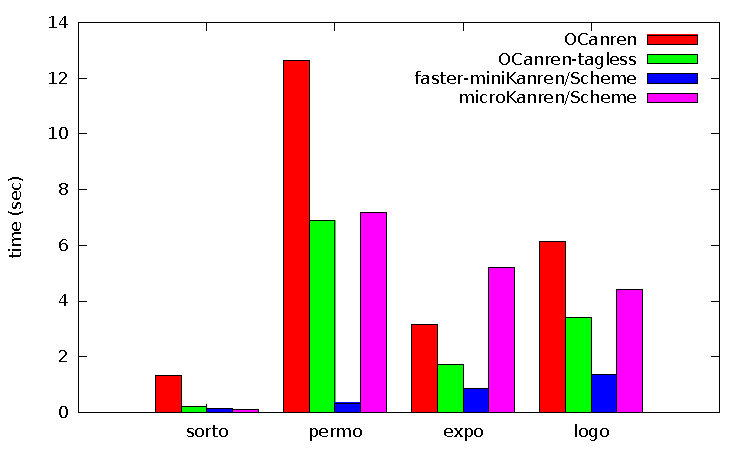
\includegraphics{graph1.pdf}
\caption{The First Set of Benchmarks}
\label{eval:first}
\end{figure}

\begin{figure}[h]
\centering
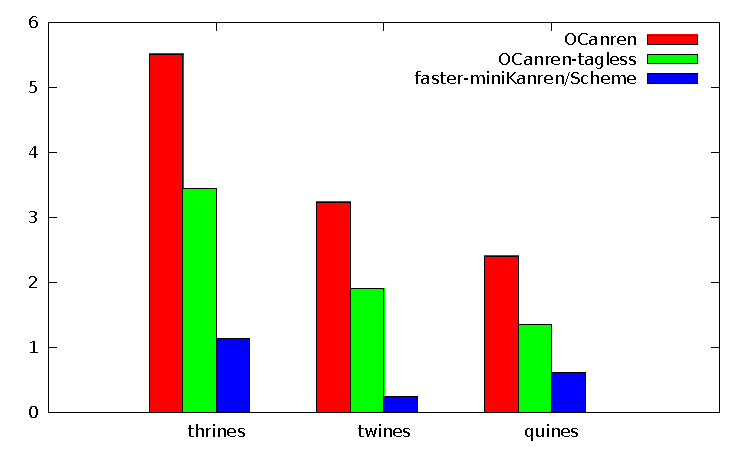
\includegraphics{graph2.pdf}
\caption{The Second Set of Benchmarks}
\label{eval:second}
\end{figure}

\section{Conclusion}

We presented a strongly-typed implementation of \miniKanren for OCaml. Our implementation
passes all tests written for \miniKanren (including those for disequality constraints);
in addition we implemented many interesting relational programs known from
the literature. We claim that our implementation can be used both as a convenient
relational DSL for OCaml and an experimental framework for future research in the area of
relational programming.

%We also want to express our gratitude to William Byrd, who infected us with relational programming,
%and for the extra time he sacrificed as both our tutor and friend.


\section{Appendix}
%% Autogenerated 12 May, 2020 19:50:32

\begin{lstlisting}
(* A|B|C *)
match ... with
| A -> 1 
| B -> 1 
| C -> 0 
\end{lstlisting}

\begin{lstlisting}
(* bool *)
match ... with
| true -> 1 
| false -> 0 
\end{lstlisting}

\begin{lstlisting}
(* bool*bool *)
match ... with
| pair (true, _) -> 1 
| pair (_, true) -> 1 
| pair (false, false) -> 0 
\end{lstlisting}

\begin{lstlisting}
(* bool*bool*bool (Maranget;page1) *)
match ... with
| triple (_, false, true) -> 1 
| triple (false, true, _) -> 2 
| triple (_, _, false) -> 3 
| triple (_, _, true) -> 4 
\end{lstlisting}

\begin{lstlisting}
(* simple lists (from Maranget2008) *)
match ... with
| pair (nil, _) -> 10 
| pair (_, nil) -> 20 
| pair (cons (_, _), cons (_, _)) -> 30 
\end{lstlisting}

\begin{lstlisting}
(* simple nats (a la Maranget2008) *)
match ... with
| pair (succ (_), succ (_)) -> 30 
| pair (zero, _) -> 10 
| pair (_, zero) -> 10 
\end{lstlisting}

\begin{lstlisting}
(* two-nil lists (with cons) *)
match ... with
| pair (nil, _) -> 10 
| pair (_, nil) -> 20 
| pair (nil2, _) -> 30 
| pair (_, nil2) -> 40 
| pair (cons (_, _), cons (_, _)) -> 60 
\end{lstlisting}

\begin{lstlisting}
(* two-nil lists (with cons; simplified RHS) *)
match ... with
| pair (nil, _) -> 10 
| pair (_, nil) -> 10 
| pair (nil2, _) -> 10 
| pair (_, nil2) -> 10 
| pair (cons (_, _), cons (_, _)) -> 60 
\end{lstlisting}

\begin{lstlisting}
(* two-nil lists (with cons; simplified RHS) *)
match ... with
| pair (nil, _) -> 10 
| pair (_, nil) -> 10 
| pair (nil2, _) -> 10 
| pair (_, nil2) -> 10 
| pair (cons (_, _), cons (_, _)) -> 60 
\end{lstlisting}

\begin{lstlisting}
(* two-nil lists (with cons; simplified RHS) *)
match ... with
| pair (nil, _) -> 10 
| pair (_, nil) -> 10 
| pair (nil2, _) -> 10 
| pair (_, nil2) -> 10 
| pair (cons (_, _), cons (_, _)) -> 60 
\end{lstlisting}

 


\begin{comment}
%% Acknowledgments
\begin{acks}                            %% acks environment is optional
                                        %% contents suppressed with 'anonymous'
  %% Commands \grantsponsor{<sponsorID>}{<name>}{<url>} and
  %% \grantnum[<url>]{<sponsorID>}{<number>} should be used to
  %% acknowledge financial support and will be used by metadata
  %% extraction tools.
  This material is based upon work supported by the
  \grantsponsor{GS100000001}{Russian Foundation for Basic Research}{https://www.rfbr.ru/rffi/eng} under Grant
  No.~\grantnum{GS100000001}{18-01-00380} and by the grant from JetBrains Research. 
  %Any opinions, findings, and
  %conclusions or recommendations expressed in this material are those
  %of the author and do not necessarily reflect the views of the
  %National Science Foundation.
\end{acks}
\end{comment}

\bibliography{references}

\end{document}
